\documentclass[twocolumn, amsmath, amsfonts, amssymb]{aastex62}
\usepackage{mathtools}
\usepackage{natbib}
\usepackage{bm}
\newcommand{\vdag}{(v)^\dagger}
\newcommand\aastex{AAS\TeX}
\newcommand\latex{La\TeX}


\newcommand{\Div}[1]{\ensuremath{\nabla\cdot\left( #1\right)}}
\newcommand{\DivU}{\ensuremath{\nabla\cdot\bm{u}}}
\newcommand{\angles}[1]{\ensuremath{\left\langle #1 \right\rangle}}
\newcommand{\KS}[1]{\ensuremath{\text{KS}(#1)}}
\newcommand{\KSstat}[1]{\ensuremath{\overline{\text{KS}(#1)}}}
\newcommand{\grad}{\ensuremath{\nabla}}
\newcommand{\RB}{Rayleigh-B\'{e}nard }
\newcommand{\stressT}{\ensuremath{\bm{\bar{\bar{\Pi}}}}}
\newcommand{\lilstressT}{\ensuremath{\bm{\bar{\bar{\sigma}}}}}
\newcommand{\nrho}{\ensuremath{n_{\rho}}}
\newcommand{\approptoinn}[2]{\mathrel{\vcenter{
	\offinterlineskip\halign{\hfil$##$\cr
	#1\propto\cr\noalign{\kern2pt}#1\sim\cr\noalign{\kern-2pt}}}}}

\newcommand{\appropto}{\mathpalette\approptoinn\relax}
\newcommand{\pro}{\ensuremath{\mathcal{P}_{\text{Ro}}\,}}


%% Tells LaTeX to search for image files in the 
%% current directory as well as in the figures/ folder.
\graphicspath{{./}{figs/}}


\received{\today}
\revised{\today}
\accepted{\today}
\submitjournal{ApJ}

\shorttitle{Predicting convective rotational constraint}
\shortauthors{Anders et al.}

\begin{document}
\defcitealias{anders&brown2017}{AB17}
\newcommand{\AB}{\citetalias{anders&brown2017}}

\title{Predicting the rotational constraint in stratified, compressible convection}

\correspondingauthor{Evan H. Anders}
\email{evan.anders@colorado.edu}

\author{Evan H. Anders}
\affil{Dept. Astrophysical \& Planetary Sciences, University of Colorado -- Boulder, Boulder, CO 80309, USA}
\affil{Laboratory for Atmospheric and Space Physics, Boulder, CO 80303, USA}
\author{Cathryn M. Manduca}
\affil{Laboratory for Atmospheric and Space Physics, Boulder, CO 80303, USA}
\author{Benjamin P. Brown}
\affil{Dept. Astrophysical \& Planetary Sciences, University of Colorado -- Boulder, Boulder, CO 80309, USA}
\affil{Laboratory for Atmospheric and Space Physics, Boulder, CO 80303, USA}
\author{Jeffrey S. Oishi}
\affiliation{Department of Physics and Astronomy, Bates College, Lewiston, ME 04240, USA}
\author{Geoff Vasil}
\affiliation{University of Sydney School of Mathematics and Statistics, Sydney, NSW 2006, Australia}


\begin{abstract}
Here we study numerical simulations of stratified, compressible convection in a
rotational $f$-plane geometry. We discuss how the rotational constraint,
measured by the Rossby number (Ro), can vary as a function of the convective driving,
measured by the Rayleigh number (Ra). We define a relationship between Ra and the
Taylor number (Ta) which we call the Predictive Rossby Number, 
\pro = Ra / Ta$^{3/4}$, and we find that the Ro remains roughly constant
across orders of magnitude of Ra when \pro is fixed. 
\end{abstract}

\keywords{convection --- happy caterpillars}

%%%%% Body of the paper
\section{Introduction}
\label{sec:intro}
Convective flows in stars and planets are influenced by rotation. 
Rotating convection has been studied in great detail in
recent decades in both laboratory and numerical settings. The
properties of convection in the regime in which rotational forces are
insignificant are now well understood \citep{king&all2009, zhong&all2009, 
cheng&all2015}. Boussinesq convective theory is also robust
in the rapidly rotating regime \citep{julien&all2012, stellmach&all2014,
gastine&all2016}. We are not, however, aware of any well-developed
procedure for specifying the degree of rotational constraint
in a convective experiment \emph{a priori}. Rather, the rotational
constraint, measured by the evolved Rossby number
(Ro, the ratio of advective dynamics to rotational constraint), is a complex
combination of input parameters, such as convective driving and the
magnitude of the rotation vector.

A vast number of studies of rotating convection have been conducted in the astrophysical context.
Often these studies focus on questions inspired by the solar dynamo
\citep{glatzmaier&gilman1982, busse2002, brown&all2008,
brown&all2010, brown&all2011, augustson&all2012, guerrero&all2013, kapyla&all2014}.
Even when these simulations appear to be rotating at a rate similar to the Sun,
they can produce vastly different dynamics (such as anti-solar differential rotation).
These strange results may be the result of these systems having different evolved
values of the Rossby number than the Sun. Recent simulations and experiments are predicting
that the Rossby number of the deep interior of the Sun is low, and that this drastically
affects the behavior of the dynamics of the solar convection zone
\citep{featherstone&hindman2016, greer&all2016}.

In addition to it being very important to study the correct Rossby number
regime in solar convection studies, it also seems to be very important in
studies of planetary dynamos. For example, the balance between Lorentz forces
and rotational forces likely creates the observed differences between ice
giant and gas giant dynamos in our solar system \citep{soderlund&all2015}.
Furthermore, \cite{aurnou&king2017} suggest that many studies in planetary systems
have likely over-emphasized the importance of magnetism compared to rotation.

\begin{figure*}[t!]
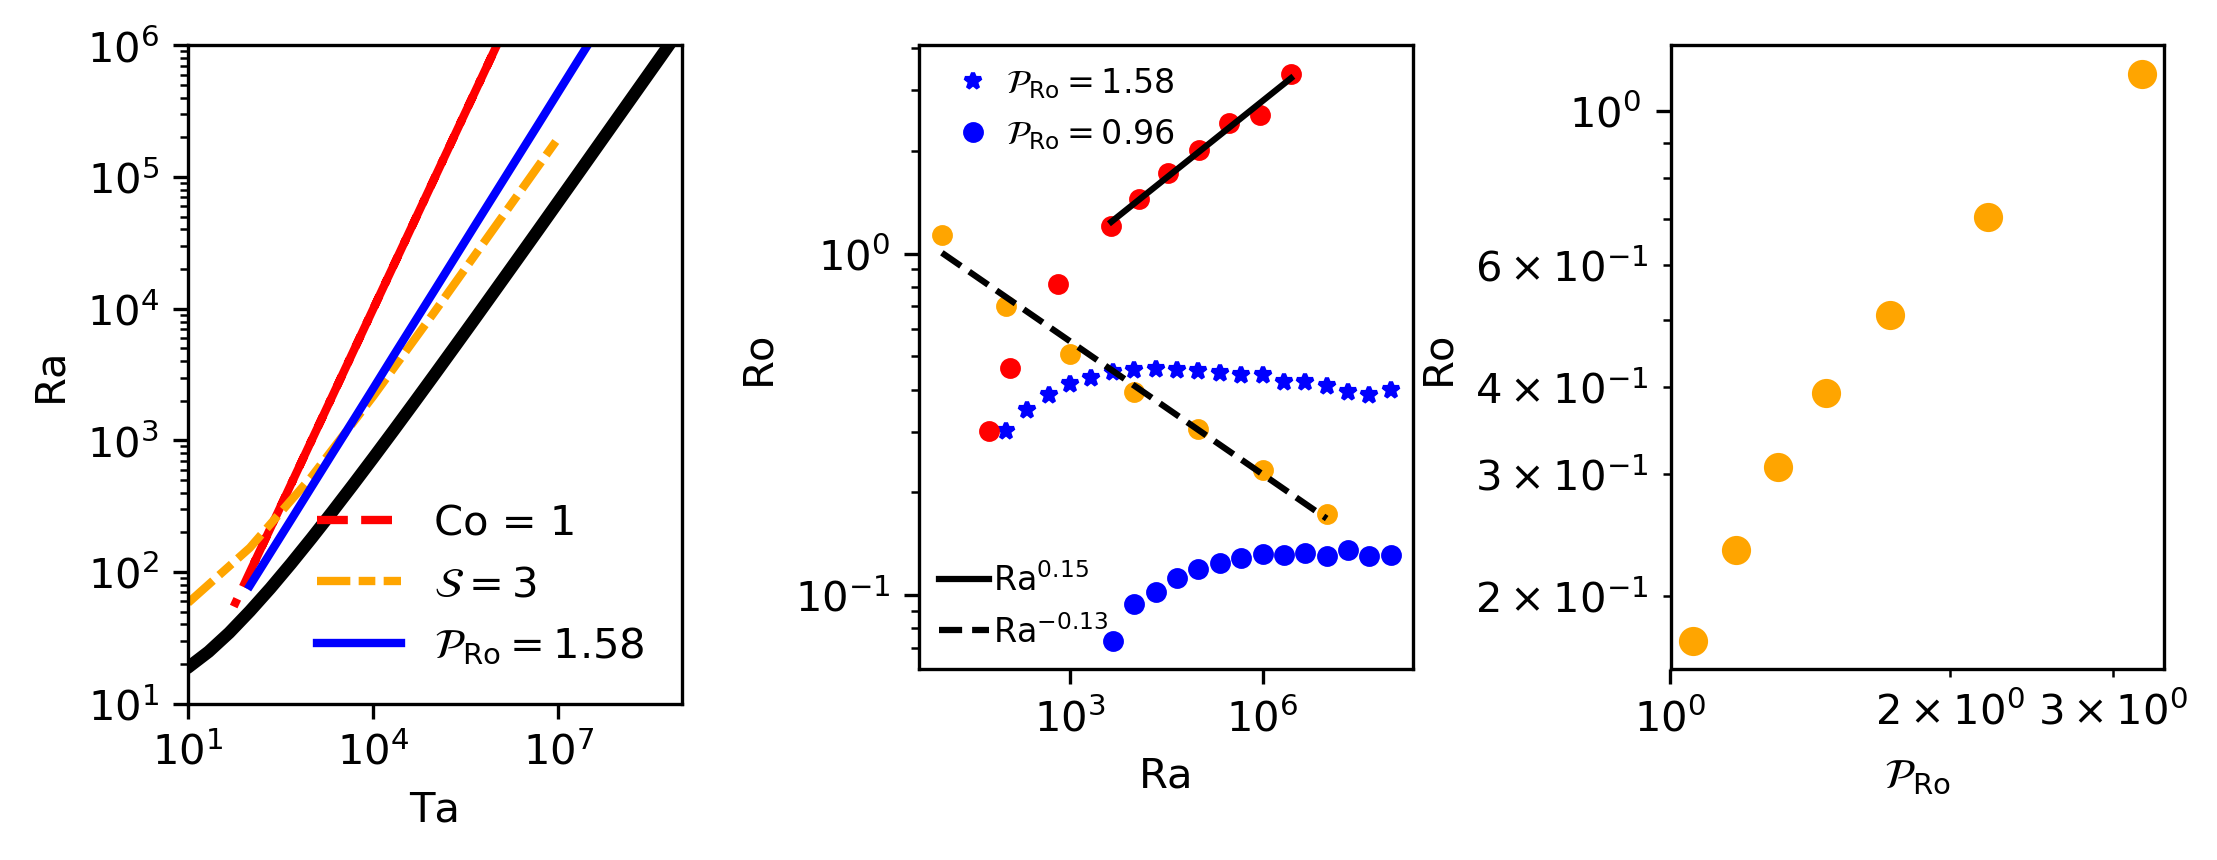
\includegraphics[width=\textwidth]{./figs/parameter_space.png}
\caption{(a) The critical Rayleigh number, as a function of the Taylor number, 
is plotted as a solid black line. Paths of constant Convective Rossby Number
(red dashed line), constant supercriticality (orange dashed line), and 
\pro (blue solid line) are shown through parameter space. (b) Evolved
Ro is plotted vs. Ra along multiple constant \pro
paths and the constant Co and $\mathcal{S}$ path shown in (a).
After a sharp increase at low Ta, the evolved Rossby number flattens
out and stays nearly constant across orders of magnitude of Ta.
(c) At low Ro, we find that $\text{Ro} \propto \pro^X$.
\label{fig:parameter_space} }
\end{figure*}


It is clear that in studying astrophysical objects, the experimenter must 
study the proper Rossby number regime, and thus the proper degree of rotational
constraint.  In this work, our goal is to find a way of specifying the Rossby number
of convection in a simplified system through changing the input parameters.
In \cite{anders&brown2017} (hereafter \AB), we studied non-rotating, hydrodynamic, 
compressible convection in polytropic atmospheres. 
In this work, we extend the study of \AB$\,$ to rotationally-influenced, $f$-plane
atmospheres, as have been previously studied by e.g.,
\cite{brummell&all1996, brummell&all1998, calkins&all2015a}. Our goal is to determine
how the input parameters which we studied previously (which control the Mach number and
Reynolds number of the evolved flows) couple with a new input
parameter, the Taylor number (Ta, \cite{julien&all1996}), which sets the magnitude of the
rotational vector. 

In section  \ref{sec:experiment}, we describe our atmosphere, numerical
experiment, and paths through parameter space. In section \ref{sec:results}, we present
the results of our experiments and in section \ref{sec:discussion} we offer concluding remarks.

\section{Experiment} 
\label{sec:experiment}


We study fully compressible, stratified 
convection under precisely the same atmospheric model
as we previously did in \AB, but here
we have included rotation. We study polytropic atmospheres
with $n_\rho = 3$ density scale heights and a superadiabatic
excess of $\epsilon = 10^{-4}$ such that flows are at low Mach number.
As in previous work \citep{julien&all1996, brummell&all1996}, 
we study a domain in which the
gravity, $\bm{g} = -g\hat{z}$, and rotational vector, $\bm{\Omega} = \Omega \hat{z}$, 
are antiparallel.

We evolve the velocity ($\bm{u}$), temperature ($T$), and log density ($\ln\rho$) according to the
Fully Compressible Navier-Stokes equations in the same form presented in \AB, with the
addition of the Coriolis term, $2\bm{\Omega}\times\bm{u}$, to the left-hand side
of the momentum equation.

\begin{figure*}[t!]
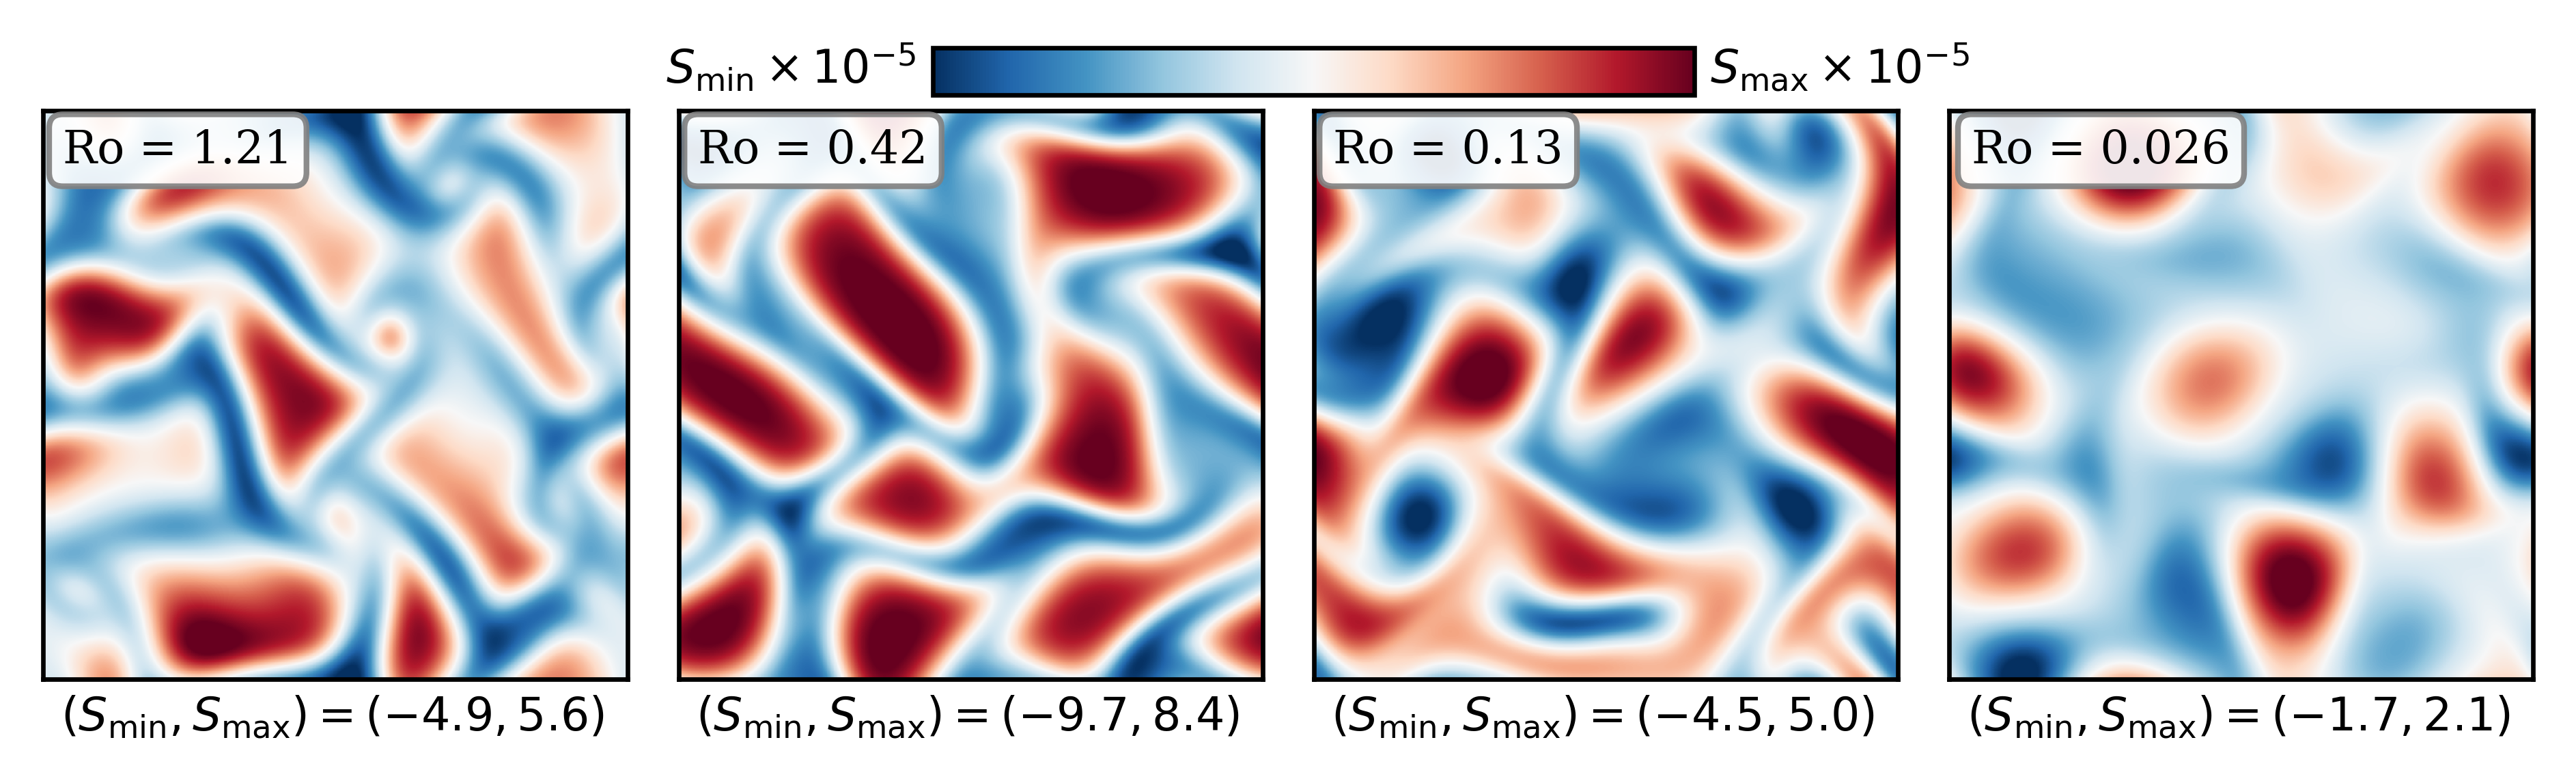
\includegraphics[width=\textwidth]{./figs/dynamics_plot.png}
\caption{ A horizontal slice of the evolved entropy field is plotted at $z = 0.95L_z$
for select simulations. The mean value of entropy at this height has been removed in all
cases. All runs displayed here have an evolved volume-averaged Ro$\,\sim\,200$. 
As Ro decreases O(1) on the left to O(0.1) on the right, and thus the rotational
constraint on the flow increases, significant changes in flow morphology are observed.
At Ro = 2.01, convective dynamics are not hugely dissimilar from the non-rotating
case where there are large upflows and narrow, fast downflow lanes (see e.g., \AB).
As the rotational constraint increases, the granular convective pattern gives way
to vortical columns, as seen at Ro = 0.13.
\label{fig:pretty_convection} }
\end{figure*}


The kinematic viscosity ($\nu$), thermal diffusivity ($\chi$), and strength of
rotation ($\Omega$) are set at the top of the domain by the Rayleigh number
(Ra), Prandtl number (Pr), and Taylor number (Ta),
\begin{equation}
\text{Ra} = \frac{g L_z^3 \Delta S / c_P}{\nu \chi}, \,\,\,
\text{Pr} = \frac{\nu}{\chi}, \,\,\,
\text{Ta} = \left(\frac{2 \Omega L_z^2}{\nu}\right)^2,
\end{equation}
where $L_z$ is the depth of the domain, 
$\Delta S = \epsilon n_\rho / m$ is the specific entropy difference between
$z = 0$ and $z = L_z$, and the specific heat at constant pressure is $c_P$.
Throughout this work we set Pr = 1.

As Ta increases, the critical value of Ra at which convection onsets,
Ra$_{\text{crit}}$, also increases (see the black line in Fig. \ref{fig:parameter_space}a). 
The linked nature of these crucial
control parameters makes it difficult to predict the rotational constraint of the evolved
fluid flows for a given set of input parameters. In this work, we will
explore three paths through Ra-Ta space:
\begin{equation}
\text{Ra} = 
\begin{cases}
\mathcal{S}\,\text{Ra}_\text{crit}(\text{Ta}), & (\text{I})\\
\text{Co}^2\text{Pr Ta}, & (\text{II}) \\
\pro^2 \text{Pr Ta}^{3/4} & (\text{III}).
\end{cases}
\label{eqn:paths}
\end{equation}
Paths on constraint I are at constant supercriticality, $\mathcal{S}$
(orange dash-dot line in Fig. \ref{fig:parameter_space}a).
Paths on constraint II are at a constant value of the classic
``Convective Rossby number'' (Co), which has been used frequently over the past
two decades, and is intended to predict the rotational constraint of the
evolved solution (red line in Fig. \ref{fig:parameter_space}a; 
\citet{julien&all1996, brummell&all1996}). Paths on constraint
III set constant a ratio which we call the ``Predictive Rossby Number'' (\pro).
These paths follow contours of Ta$^{3/4}$, and to our knowledge have not been
well-explored in the literature (blue solid line in Fig. \ref{fig:parameter_space}a).  




In this work, our goal is to study the magnitude of the rotational constraint
along each path defined in Eqn. \ref{eqn:paths}. We will quantify rotational
constraint using the Rossby number,
\begin{equation}
\text{Ro} = \frac{|\grad\times \bm{u}|}{2 \Omega}.
\label{eqn:ro}
\end{equation}

As Ta increases, the wavenumber of convective onset, $k_{\text{crit}}$, also increases. 
We study 3D cartesian convective domains with horizontal extents of
$x, y = [0, 4(2\pi/k_{\text{crit}})]$. 
We evolve our simulations using the Dedalus\footnote{\url{http://dedalus-project.org/}} 
pseudospectral framework, and our numerical methods are identical to those presented
in \AB.



\section{Results \& Discussion}

\label{sec:results}
In Fig.~\ref{fig:parameter_space}a, we display the value of the critical Rayleigh number 
(Ra$_{\text{crit}}$) as a function of the Taylor number (Ta). We found these critical
values through the use of a linear instability analysis. We plot a sample path for
each criterion in Eqn. \ref{eqn:paths} through
this parameter space.
In Fig. \ref{fig:parameter_space}b, we show that along paths of
constant $\mathcal{S}$, Ro 
decreases as a function of Ra and Ta. Along paths of constant Co, Ro increases
with increasing Ra and Ta. However, along paths of constant \pro, 
after an increase at low Ra, the evolved value of Ro levels off and stays roughly constant
as a function of Ra. Holding \pro constant seems to predict Ro relatively
well from our experimental trials here, particularly at low Ro. 
In Fig. \ref{fig:parameter_space}c, we
show how the Ro varies as a function of \pro at constant supercriticality.
We expect the scaling law for Ro $\leq 0.4$ to hold up to low Ro, and the
leveling off seen at higher Ro and higher \pro is likely influenced by the
curvature of the supercriticality curve at low Ra and Ta (see Fig. \ref{fig:parameter_space}a).


In Fig.~\ref{fig:pretty_convection}, we show sample snapshots of the evolved entropy field
near the top of the domain. The cases displayed have evolved Ro spanning roughly an order
of magnitude. As we study the increasingly rotationally constrained regime, we see the
classic granular structure of convection (see e.g., Fig.~2 in \AB) give way to vortical
columns of convection, as seen in rapidly rotating \RB convection \citep{stellmach&all2014}.
All cases displayed in Fig.~\ref{fig:pretty_convection} have an evolved volume-averaged
Re of roughly 200.


\begin{figure}[h]
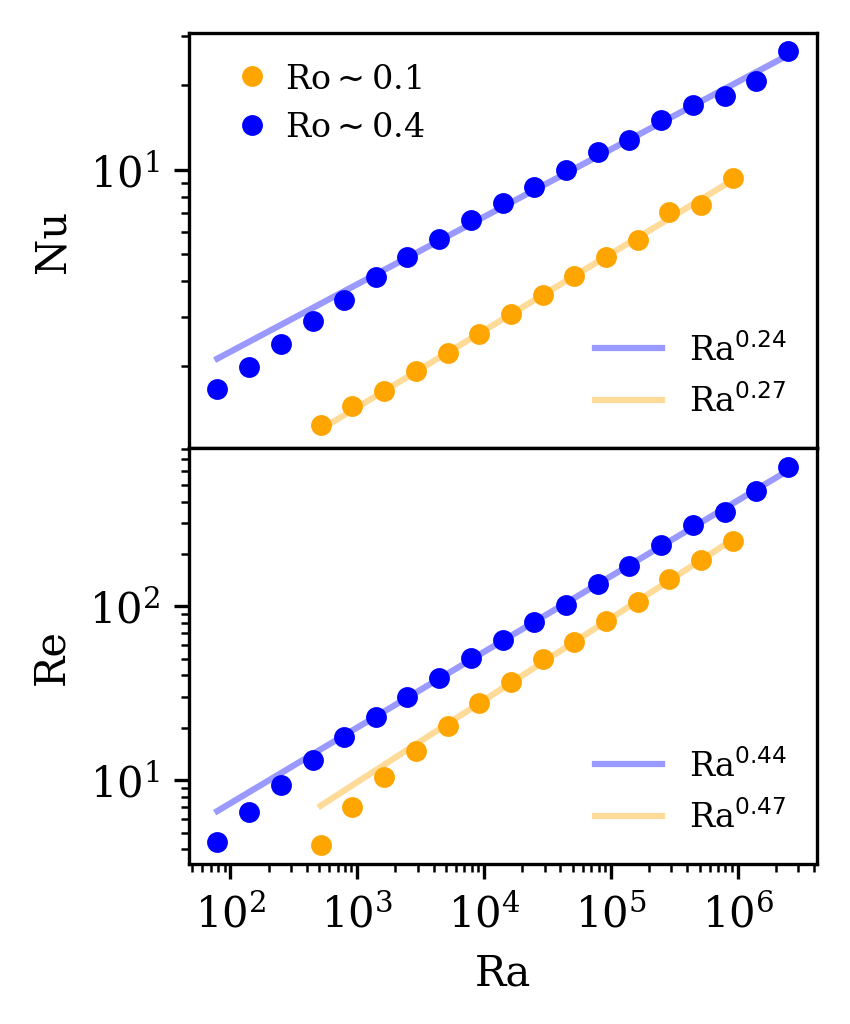
\includegraphics{./figs/nu_and_re.png}
\caption{(a) Evolved Nu vs. Ra along constant
\pro$\,$ paths. A scaling law of Nu$\,\propto\,$Ra$^{0.27}$ is observed, which
is very similar to classic scaling laws.
(b) Evolved Re vs. Ra along constant \pro$\,$ paths.
A classic scaling law of Re$\,\propto\,$Ra$^{1/2}$ is observed. The
similarity between these laws and
classical laws in \RB convection suggests that at fixed \pro, varying Ra
affects the evolved dynamics in a manner similar to a nonrotating fluid.
\label{fig:nu_and_re} }
\end{figure}

We define the Nusselt number (Nu, which quantifies heat transport in a convective
solution) as we did previously in \AB.
In Fig. \ref{fig:nu_and_re}a, we show the scaling of Nu as a function
of Ra at fixed \pro. We find that when \pro$\,$ is held constant and
Ra is increased, we find a scaling of $\text{Nu} \propto \text{Ra}^{0.27}$,
which is reminiscent of classical scaling laws in non-rotating theory,
and suggests that changes in heat transport along these paths are boundary
driven. Furthermore, in Fig. \ref{fig:nu_and_re}b, we plot the RMS Reynold's
number (Re $= |u| L_z / \nu$) as a function of Ra, and find that 
$\text{Re} \propto \text{Ra}^{1/2}$, which is precisely the scaling we found
in the non-rotating regime in \AB.


\begin{figure*}[h]
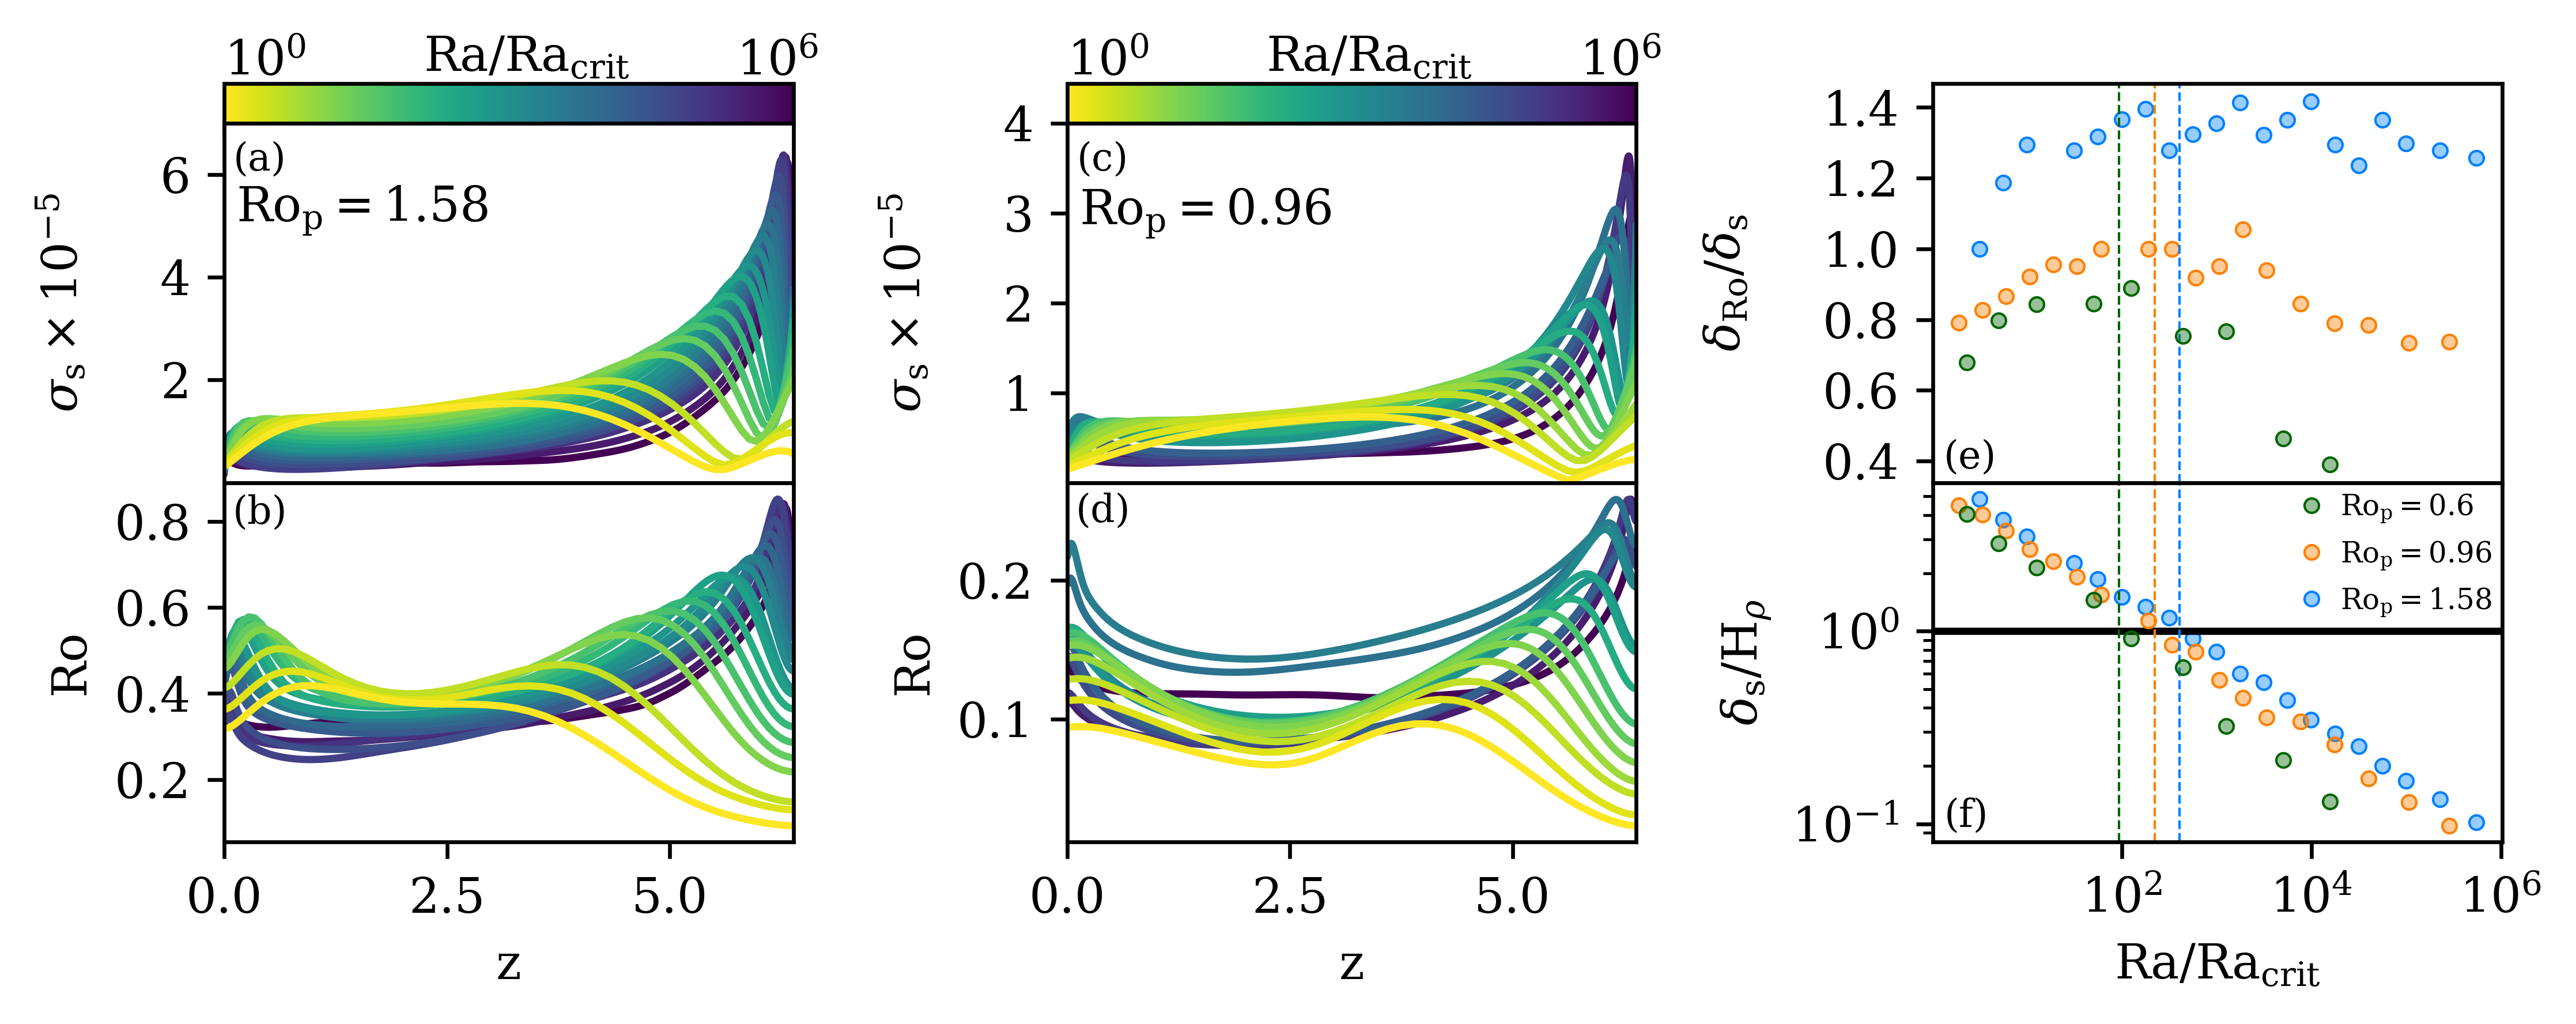
\includegraphics[width=\textwidth]{./figs/boundary_layers.png}
\caption{(a) Horizontally-averaged profiles of the Rossby number are shown
vs. z for a constant \pro$\,$ = X. (b) Horizontally-averaged profiles of 
the entropy gradient are shown vs. z for a constant \pro$\,$ = X.
(c) Vorticity boundary layer thickness normalized by entropy boundary layer
thickness as a function of Ta/Ta\_crit for multiple \pro$\,$ paths.
When this measure is $\gg 1$, we expect the flows to be buoyancy dominated,
when it is $\ll 1$, we expect the flows to be rotationally dominated,
and when it is $\sim 1$, we anticipate that both effects are very important.
\label{fig:profiles_and_bls} }
\end{figure*}

In Fig. \ref{fig:profiles_and_bls}, we show time- and horizontally-averaged profiles of
the rossby number and the entropy gradient. As Ra increases at a constant value of
\pro, both the entropy and rotational boundary layers shrink. We measure the
upper boundary layer thicknesses of both profiles. We measure the boundary layer thickness
of the Rossby number as the distance from the upper boundary to the point at which Ro
is maximized. We measure the boundary layer thickness of the entropy profile by fitting
a line to the upper 10 points in the domain, and assuming that the boundary layer extends to
the point at which that line crosses through zero. We plot $\delta_S/\delta_{\text{Ro}}$
as a function of Ra for our \pro$\,$ paths in Fig. \ref{fig:profiles_and_bls}b. We find
that the ratio of these boundary layers is relatively constant as a fucntion of Ra, which
implies that the rotational constraint across Ra is roughly constant.
[NOTE: NEED TO TALK ABOUT MAGNITUDE OF RO IN BOUNDARY LAYER]

\section{Discussion}
\label{sec:discussion}
In this letter, we studied rotating, stratified, compressible convection at low Mach 
number. We studied traditional paths through Ra-Ta space, as well as a new path,
in which the Predictive Rossby number, \pro, is held constant, and
$\text{Ra} = \pro \text{Ta}^{3/4}$. Along these paths, we find that the evolved
rotational constraint, as measured by the Rossby number (Ro), is roughly constant as
Ra increases. Furthermore, the heat transport, measured by the Nusselt number (Nu), and the
level of turbulence, as measured by the Reynolds number (Re), vary according to traditional 
scaling laws as Ra increases. Together, these phenomena suggest that experimenters in
stratified convection can specify the degree of rotational constraint in their evolved
solutions by choosing \pro$\,$, and then increase Ra in a manner analogous to 
unrotating convection (e.g., \AB) to increase the efficiency and turbulent nature of the
convective dynamics in question.







\subsection{acknowledgements}
EHA acknowledges the support of the University of Colorado's George 
Ellery Hale Graduate Student Fellowship.
This work was additionally supported by  NASA LWS grant number NNX16AC92G.  
Computations were conducted 
with support by the NASA High End Computing (HEC) Program through the NASA 
Advanced Supercomputing (NAS) Division at Ames Research Center on Pleiades
with allocations GID s1647.

\bibliography{biblio.bib}
\end{document}
